\documentclass[12pt]{article}
\usepackage[utf8]{inputenc}
\usepackage[paper=letterpaper,margin=2cm]{geometry}
\usepackage{amsmath, array}
\usepackage{amssymb}
\usepackage{amsfonts}
\usepackage{enumitem}
\usepackage{titling}
\usepackage[spanish]{babel}
\decimalpoint
\usepackage[colorlinks=true]{hyperref}
\usepackage{listingsutf8}
\usepackage[pdftex]{graphicx}
\usepackage{caption}
\usepackage{subcaption}
\usepackage{fancyhdr}
\usepackage{multirow}
\usepackage{biblatex}
\usepackage{physics}
\usepackage{siunitx}

\usepackage[table,xcdraw,dvipsnames]{xcolor}
\addbibresource{ref.bib}
\usepackage{tocloft}
\hypersetup{linkcolor=blue}
\newcommand{\m}{\text{m}}
\newcommand{\mpers}{\unit[per-mode = symbol]{\metre\per\second}}
\definecolor{codegreen}{rgb}{0,0.5,0}
\pagestyle{fancy}
\fancyhf{}

\title{Plantilla prácticas}
\author{Rodrigo Rafael Castillo Chong}
\date{\today}
\begin{document}
\lstset{inputencoding=utf8/latin1}
\lstdefinestyle{myStyle}{
	keywordstyle=\color{blue},
	commentstyle=\color{codegreen},
	backgroundcolor=\color{gray!10!white},
}
\lstset{style=myStyle}
	\thispagestyle{empty}
	
	\begin{figure}[ht]
		\minipage{0.7\textwidth}
		
\includegraphics[width=4cm]{images/usaclogo.png}
		\label{EscudoUSAC}
		\endminipage
		\minipage{0.32\textwidth}
		
\includegraphics[height = 4cm ,width=4cm]{images/logoecfmplain.png}
		\label{EscudoECFM}
		\endminipage
	\end{figure}
	
	\begin{center}
		\vspace{0.8cm}
		\LARGE
		UNIVERSIDAD DE SAN CARLOS DE GUATEMALA
		
		\vspace{0.8cm}
		\LARGE
		ESCUELA DE CIENCIAS FÍSICAS Y MATEMÁTICAS
		
		\vspace{1.7cm}	
		\Large
		\textbf{Informe final de prácticas}
		
		\vspace{1.7cm}
		\Large
		\textbf{Evaluación de distintos métodos numéricos para resolver ecuaciones particulares de la mecánica de fluidos}
		
		
		\vspace{1.3cm}
		\normalsize	
		POR \\
		\vspace{.3cm}
		\large
		\textbf{Rodrigo Rafael Castillo Chong \\ 201804566}
		
		\vspace{1.3cm}
		\normalsize	
		ASESORADO POR \\
		\vspace{.3cm}
		\large
		\textbf{Enrique Pazos, Ph.D.}
		
		
		
		\vspace{1.3cm}
		\today
	\end{center}
	
	\newpage
	\tableofcontents
	\clearpage
	
	\section{Método de diferencias finitas}
	El \textbf{método de diferencias finitas} o \textbf{método DF} es un método numérico que sirve para resolver ecuaciones diferenciales ordinarias o parciales. El método consiste en discretizar el dominio de la ecuación en un conjunto finito de puntos llamado \textbf{grilla}; donde cada punto debe estar a la misma distancia de cada uno de sus vecinos. Posteriormente se deben aproximar las derivadas de la función con ecuaciones de diferencias utilizando series de potencias, para poder resolver la ecuación diferencial algebraica e iterativamente \cite{devries2011first}.
	
	Un ejemplo de discretización, que se usa al aplicar el método DF en una ecuación diferencial parcial, es el siguiente: la segunda derivada parcial respecto a $x$ de una función $u = u(x,t)$ valuada en $(x,t)$ se puede aproximar expandiendo la función en dos series de Taylor centradas en dos diferentes valores sobre el eje $x$, que corresponden a los dos puntos vecinos a $x$, separándose de este punto por una distancia $\Delta x$; también llamada \textbf{tamaño de paso} en $x$. 
	
	Para obtener la aproximación de la segunda derivada de $u$ respecto a $x$ usamos las expansiones en series de Taylor:

	\begin{equation}
		u(x + \Delta x,t) \approx u(x,t) + \Delta x\pdv{u}{x}+ \frac{(\Delta x)^{2}}{2}\pdv{^{2}u}{x^2} 
	\end{equation}

	\begin{equation}
		u(x - \Delta x,t) \approx u(x,t) - \Delta x\pdv{u}{x}+\frac{(\Delta x)^{2}}{2}\pdv{^{2}u}{x^2} 
	\end{equation}
	Sumando ambas aproximaciones se obtiene:
	\begin{equation}
		(\Delta x)^2 \pdv{^{2}u}{x^2}\approx u(x + \Delta x,t) + u(x - \Delta x,t) - 2 u(x,t)
	\end{equation}

	\begin{equation}
		\pdv{^{2}u}{x^2}\approx \frac{u(x + \Delta x,t) + u(x - \Delta x,t) - 2 u(x,t)}{(\Delta x)^2}
	\end{equation}
	Por tanto, podemos aproximar una derivada de segundo orden en términos de valores conocidos, puesto que $u(x + \Delta x,t)$ y $u(x - \Delta x,t)$ corresponden a valores que toma la función en un dominio discretizado, en donde la distancia entre los puntos de la grilla es siempre $\Delta x$. Se puede escribir la función valuada en forma discreta:
	\[u_{i} := u(x,t)\]
	\[u_{i+1} := u(x + \Delta x,t)\]
	\[u_{i-1} := u(x - \Delta x,t)\]
	De tal forma que la aproximación de la segunda derivada parcial se puede representar de manera compacta
	\begin{equation}
		\pdv{^{2}u}{x^2} \approx \frac{u_{i+1}-2u_{i}+u_{i-1}}{(\Delta x)^{2}}
	\end{equation}
	En la figura \ref{fig:discretizacion} se observa la representación gráfica de esta discretización.
	
	\begin{figure}[ht]
		\centering
		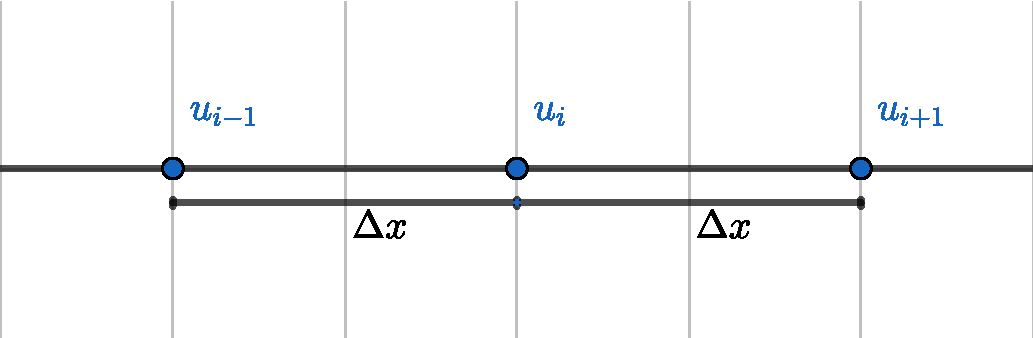
\includegraphics[scale=0.8]{images/grilla.pdf}
		\caption{Discretización del dominio espacial}
		\label{fig:discretizacion}
	\end{figure}
	
	
	En general, el dominio temporal de la función también se discretiza, tomando intervalos de tiempo consecutivos separados por un intervalo de tiempo $\Delta t$ o también llamado tamaño de paso en $t$. 
	
	\newpage
	Para aproximar la primera derivada parcial en $t$ de $u$ se expande la función en una serie de Taylor centrada en $\Delta t$ y el término donde la función está valuada en el instante temporal mayor se renombra como $u_{\text{nueva}}$.
	
	\[u(x,t+\Delta t)\approx u(x,t) + \Delta t \pdv{u}{t}\]
	\[\pdv{u}{t} \approx \frac{u(x,t+\Delta t) - u(x,t)}{\Delta t}\]
	\[\pdv{u}{t} \approx \frac{u_{\text{nueva,} i} - u_{i}}{\Delta t}\]
	
	Posteriormente se reemplazan las discretizaciones aproximadas en la ecuación diferencial a resolver y se itera sobre la relación de recurrencia encontrada para los valores actuales y futuros de la función en un punto dado. 
	
	En resumen, el método DF funciona aproximando y adaptando las derivadas de primer y segundo orden a ecuaciones de diferencias que dependen de los valores que la función devuelve cuando esta se valúa en los puntos de la grilla, o bien, en instantes discretos de tiempo.\\
	
	A continuación se describen los problemas resueltos con el método de diferencias finitas y los resultados conseguidos con este.

	
	\subsection{Ecuación de Burgers no viscosa, en una dimensión}
	\subsubsection{Descripción del problema}
	La ecuación de Burgers no viscosa en una dimensión espacial es una ecuación diferencial parcial de primer orden que expresa la evolución temporal de la cantidad $u = u(x,t)$, la cual puede ser interpretada como la componente en $x$ de la \textbf{velocidad} de un fluido o gas. La ecuación tiene la siguiente forma:
	\begin{equation}
		\pdv{u}{t}+u\pdv{u}{x}=0
		\label{eq:burgers1d}
	\end{equation}
	
	Se resolvió esta ecuación en un dominio espacial $I$ dado por $I = [0,\text{L}]$, donde $\text{L} = 100 \unit{\meter}$, y sujeta a las siguientes condiciones iniciales:\\
	\begin{equation}
		u(0,0)=0
	\end{equation}
	\begin{equation}
		u(\text{L},0)= 0
	\end{equation}
	Estas condiciones pueden interpretarse como el modelado de un fluido sin presión ni viscosidad, o un gas, que se mueve en una dimensión cuyos extremos simulan un tope o frontera que impide que el fluido o gas en cuestión salga. %Se tomó $\text{L}=100\m$ como el largo del dominio.
	
	Como condición inicial se eligió una distribución gaussiana de velocidad. Esta se puede interpretar como un pulso centrado en el centro del dominio. Es común utilizar pulsos gaussianos como condiciones iniciales, para así visualizar su desplazamiento a lo largo de la simulación\footnote{En las ecuaciones se mantuvieron los nombres de las variables utilizadas en el código de la integración numérica de la ecuación, salvo por $\mu$ que se escribió como \texttt{mu}.}.
	\begin{equation}
		u(x,0) = A\exp(-b(x-\mu)^{2})
		\label{eq:condinicial}
	\end{equation}
	\\
	Donde:
	\begin{itemize}
		\item $A=3.5\mpers$
		\item $b=0.05$
		\item $\mu=L/2=50\unit{\meter}$
	\end{itemize}

	\subsubsection{Aplicación del método y código implementado}
	Se utilizó el lenguaje \texttt{C++} para resolver el problema numérico utilizando el método de diferencias finitas. El código completo está disponible en el siguiente \href{https://github.com/highchen147/practicas/blob/main/burgers1DDF/burgers1DDF.cpp}{enlace.}
	
	
	Para resolver numéricamente la ecuación \ref{eq:burgers1d} utilizando el método DF, primero se debe discretizar el dominio en el que esta se define. Para la simulación se definió un conjunto de \texttt{Nx} puntos sobre el eje $x$ de tal manera que cada par de puntos vecinos estuvieran separados por una distancia \texttt{dx}, la cual equivale a $\Delta x$ en la simbología algebraica de este documento.
	
	\lstinputlisting[title = Valores de los parámetros para discretización del dominio espacial, language = C++,
	firstline=30,
	lastline=32,
	commentstyle=\color{codegreen},
	keywordstyle=\color{blue}]{../burgers1DDF/burgers1DDF.cpp}
	
	Es destacable que el denominador de la fracción que define a \texttt{dx} es $\texttt{Nx-1}$ dado que el intervalo contiene esta cantidad de veces la distancia \texttt{dx.} 

	Para almacenar los valores de la función $u$ se utilizaron punteros a arreglos dinámicos de tipo \texttt{\color{blue}{double}}, al igual que para almacenar el conjunto de puntos que conforma el dominio discretizado en el eje $x$. Estos también fueron inicializados dependiendo de su definición; en el caso de $u$, se aplicó la condición inicial del problema y las condiciones de frontera.	
	
	\lstinputlisting[title = Definición e inicialización de arreglos dinámicos, 
	language = C++, 
	firstline=42,
	lastline=61,
	keywordstyle=\color{blue}]{../burgers1DDF/burgers1DDF.cpp}
	
	\lstinputlisting[title = Implementación de la ecuación \ref{eq:condinicial}, 
	language = C++,
	firstnumber = 112,
	firstline=112,
	lastline=118,
	keywordstyle=\color{blue}]{../burgers1DDF/burgers1DDF.cpp}
		
	
	Para discretizar el dominio temporal se tomó \texttt{t\_total} como la variable que almacena el tiempo total a simular y \texttt{dt} como el tamaño de paso temporal; por tanto, el número de iteraciones necesarias para simular el tiempo completo se obtiene dividiendo \texttt{t\_total} entre \texttt{dt}. Sin embargo, puede que el resultado de esta división no sea un número entero, por lo que se le aplicó la función \texttt{floor()} para garantizarlo. La variable \texttt{num\_outs} es un número entero que indica cuántos instantes temporales serán impresos en el archivo de datos; esta cantidad es importante ya que la velocidad de simulación depende de qué tantas veces se imprimen los datos. Las variables de tipo \texttt{const} pueden ser cambiadas a voluntad del usuario, siempre y cuando el cambio sea efectuado en la declaración de las mismas.
	
	\lstinputlisting[title = Valores de los parámetros para discretización del dominio temporal, language = C++, 
	firstline=19, 
	lastline=27, 
	keywordstyle=\color{blue}]{../burgers1DDF/burgers1DDF.cpp}
	
	El siguiente paso para implementar el método consistió en aproximar las derivadas utilizando las discretizaciones disponibles, esto es:
	\begin{equation}
		\pdv{u}{x} \approx \frac{u(x+\Delta x,t)-u(x,t)}{\Delta x}
	\end{equation}
	\begin{equation}
		\pdv{u}{x} \approx \frac{u_{i+1}-u_{i}}{\Delta x}
	\end{equation}
	\begin{equation}
		\pdv{u}{t} \approx \frac{u_{\text{nueva},i}-u_{i}}{\Delta t}
	\end{equation}
	Donde $\Delta x$ y $\Delta t$ son los tamaños de paso en la dimensión espacial y temporal respectivamente\footnote{En el código, estas cantidades fueron nombradas como \texttt{dx} y \texttt{dt} respectivamente}. Sustituyendo las anteriores aproximaciones en \ref{eq:burgers1d}, obtenemos
	\begin{equation}
		\frac{u_{\text{nueva},i}-u_{i}}{\Delta t}+u_{i}\left( \frac{u_{i+1}-u_{i}}{\Delta x}\right) =0
	\end{equation}
	Luego se despeja $u_{\text{nueva},i}$
	\begin{equation}
		u_{\text{nueva,}i} = u_{i}\left[ 1 + \frac{\Delta t}{\Delta x}(u_{i}-u_{i+1}) \right]
		\label{eq:burgdiscr}
	\end{equation}
	De esta forma, el valor de la función $u$ en el i-ésimo elemento de la grilla, en un instante $t + \Delta t$, está dado por el miembro derecho de la ecuación \ref{eq:burgdiscr}, cuyos términos son valores de $u$ en el mismo instante $t$. Esta es una relación de recurrencia sobre la cual se puede iterar para construir la solución general de la ecuación.
	
	A continuación se muestra el ciclo principal de integración numérica de la ecuación de Burgers
	\lstinputlisting[title = Ciclo principal de integración, 
	language = C++,
	firstnumber = 71,
	firstline=71,
	lastline=94,
	keywordstyle=\color{blue}]{../burgers1DDF/burgers1DDF.cpp}
	
	Se puede notar que para realizar la integración numérica de la ecuación se necesitan anidar dos ciclos \texttt{\color{blue}{for}}, uno para iterar sobre el dominio temporal y otro para el dominio espacial. En la quinta línea se puede apreciar la implementación de la ecuación \ref{eq:burgdiscr} en código y en las líneas consecuentes se observa la asignación de las condiciones de frontera.
	
	Se utilizó una función especial llamada \texttt{salida} que toma como argumento una variable de tipo \texttt{ofstream} la cual sirve para enviar datos al archivo deseado.
	\lstinputlisting[title = Definición de función de salida de datos, 
	language = C++,
	firstline=120,
	lastline=127,
	keywordstyle=\color{blue}]{../burgers1DDF/burgers1DDF.cpp}
	\subsubsection{Resultados}
	Se graficó una animación de la simulación numérica en \textbf{Gnuplot}, una herramienta de visualización de datos ampliamente utilizada en el ámbito científico. Se encontró que después de un tiempo de simulación de $1.2\unit{\second}$, los resultados comenzaron a presentar un considerable error numérico y a perder significado físico. Sin embargo, se pudo explicar la razón de este fenómeno investigando sobre la ecuación de Burgers. En la sección \ref{sec:discusion} se discutirá con más detalle el tema del error numérico de la solución.
	
	En la figura \ref{fig:instantesB1DDF} se muestran seis instantes de la evolución temporal. La animación de la simulación completa se encuentra disponible en el siguiente \href{google.com}{enlace.}
	
	\begin{figure}[h]
		\centering
		\begin{subfigure}{0.5\textwidth}
			\centering
			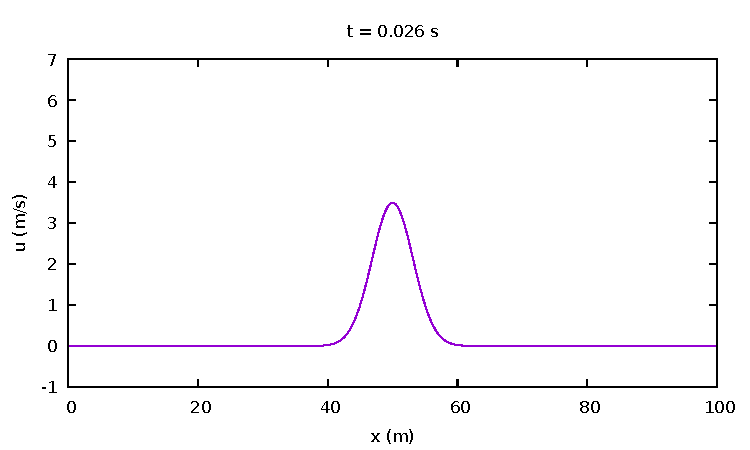
\includegraphics[width=\textwidth]{../burgers1DDF/results/frame001.pdf}
			\caption*{Gráfica de $u(x,t=0.026\unit{\second})$}
			\label{fig:b1ddf1}
		\end{subfigure}\hfill
		\begin{subfigure}{0.5\textwidth}
			\centering
			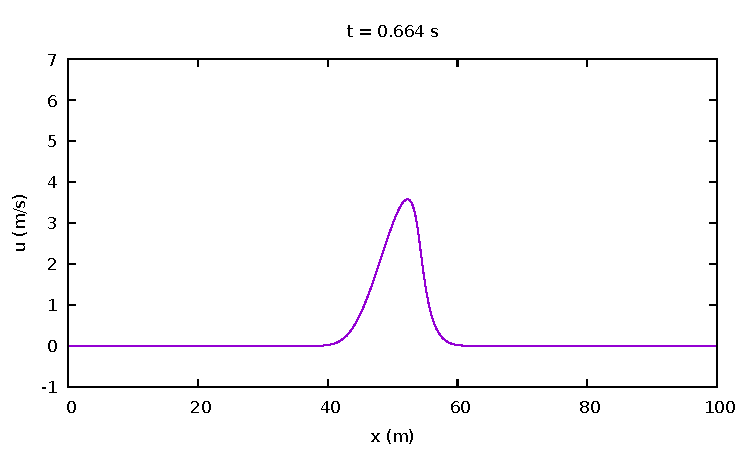
\includegraphics[width=\textwidth]{../burgers1DDF/results/frame026.pdf}
			\caption*{Gráfica de $u(x,t=0.664\unit{\second})$}
			\label{fig:b1ddf2}
		\end{subfigure}\par
		\begin{subfigure}{0.5\textwidth}
			\centering
			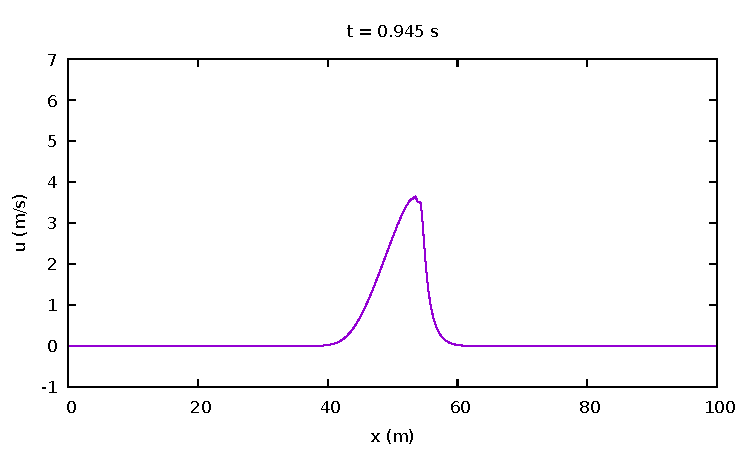
\includegraphics[width=\textwidth]{../burgers1DDF/results/frame037.pdf}
			\caption*{Gráfica de $u(x,t=0.945\unit{\second})$}
			\label{fig:b1ddf3}
		\end{subfigure}\hfill
		\begin{subfigure}{0.5\textwidth}
			\centering
			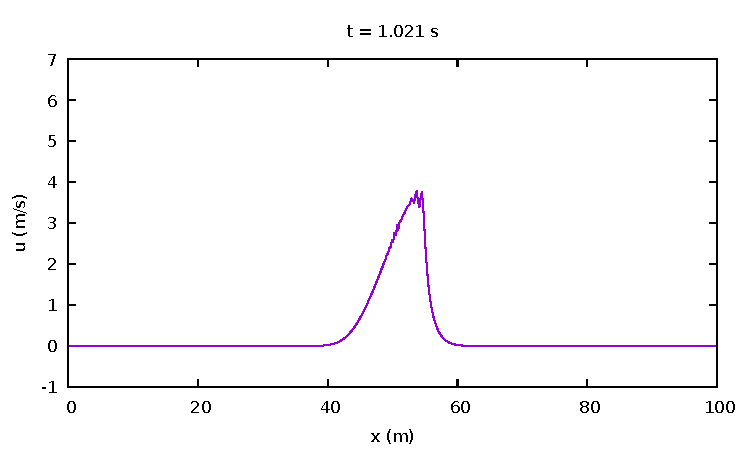
\includegraphics[width=\textwidth]{../burgers1DDF/results/frame040.pdf}
			\caption*{Gráfica de $u(x,t=1.021\unit{\second})$}
			\label{fig:b1ddf4}
		\end{subfigure}\par
		\begin{subfigure}{0.5\textwidth}
			\centering
			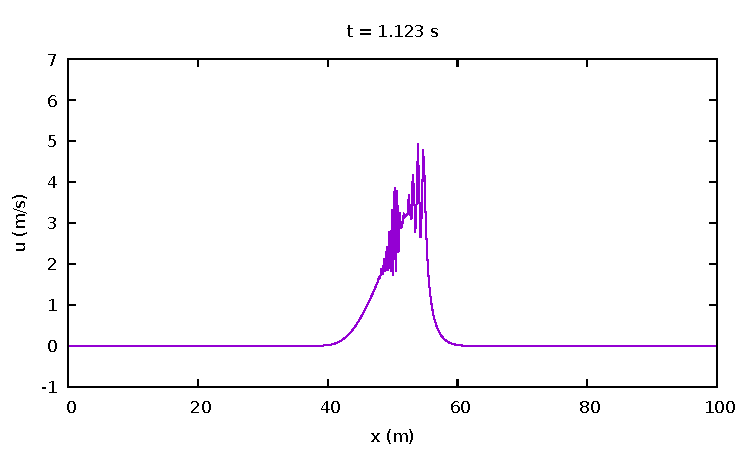
\includegraphics[width=\textwidth]{../burgers1DDF/results/frame044.pdf}
			\caption*{Gráfica de $u(x,t=1.123\unit{\second})$}
			\label{fig:b1ddf5}
		\end{subfigure}\hfill
		\begin{subfigure}{0.5\textwidth}
			\centering
			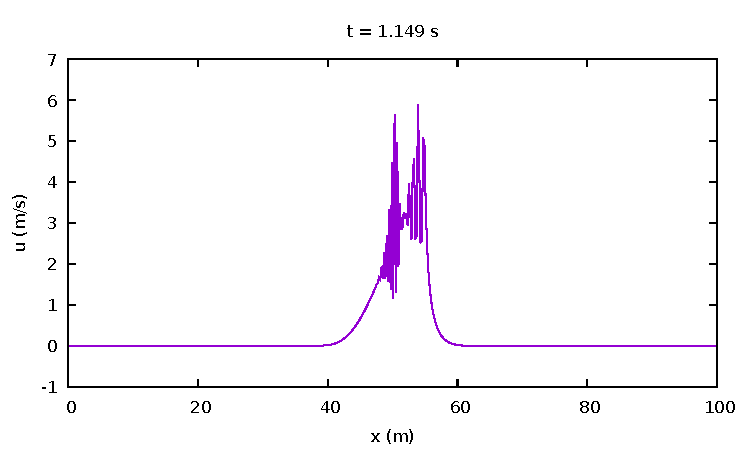
\includegraphics[width=\textwidth]{../burgers1DDF/results/frame045.pdf}
			\caption*{Gráfica de $u(x,t=1.149\unit{\second})$}
			\label{fig:b1ddf6}
		\end{subfigure}
		\caption{Seis instantes de tiempo de la evolución temporal de la ecuación de Burgers no viscosa con diferencias finitas.}
		\label{fig:instantesB1DDF}
	\end{figure}
	
	
	\subsubsection{Discusión de resultados}
	\label{sec:discusion}
	La ecuación de Burgers resuelta con el método de diferencias finitas mostró algunas irregularidades, principalmente la pérdida de continuidad en varias partes de la solución a partir del segundo $1.021$ de la simulación. Este fenómeno es causado gracias al efecto de \textbf{onda de choque}  (o \textbf{shockwave} en inglés) que la ecuación de Burgers presenta. Una onda de choque se define como una discontinuidad en la velocidad de propagación de una onda y dado que la ecuación de Burgers representa la velocidad del fluido modelado, la discontinuidad se manifiesta en la función solución de la ecuación.
	
	Para explicar el fenómeno de onda de choque que se produce en la ec. de Burgers se puede utilizar el \textbf{método de características} para la resolución de la ecuación misma. El método de características consiste en transformar el dominio de la ecuación tal que, en éste, la ecuación diferencial parcial se pueda escribir como un sistema de ecuaciones diferenciales ordinarias, llamadas \textbf{ecuaciones características}. Las curvas del dominio en donde al valuar la ecuación esta se puede escribir como un sistema de ecuaciones diferenciales ordinarias se llaman \textbf{curvas características.}
	Para encontrar las curvas características de la ec. de Burgers se necesitan resolver las ecuaciones características: 
	\begin{equation}
		\dv{x}{t} = u(x,t)
		\label{eq:dxdt}
	\end{equation}
	\begin{equation}
		\dv{u}{t} = \pdv{u}{t} + \dv{x}{t}\pdv{u}{x} = \pdv{u}{t}+u\pdv{u}{x} = 0
		\label{eq:parcialu}
	\end{equation}
	Notamos en la ecuación \ref{eq:parcialu} que $u$ es constante en el tiempo a lo largo de cualquier curva característica, por lo que resolviendo la ecuación \ref{eq:dxdt} obtenemos:
	\begin{equation}
		x-x_{0} = ut
	\end{equation}
	\begin{equation}
		x(t) = x_{0} + u_{0}(x_0)t
		\label{eq:caracteristica}
	\end{equation}
	Donde $u_0(x) = u(x,0)$
	
	Notamos que las curvas características son rectas en el plano $x-t$ que parten de un punto $(x_{n}, 0)$ y poseen pendiente $u_{0}(x_n)$, donde $x_n$ es un punto que pertenece al dominio espacial. Consecuentemente se puede demostrar que estas curvas se intersectarán en un tiempo finito si $u'_{0}(x) < 0$ para algún $x$. Supongamos que las dos características $x(t) = x_{1}+u_{0}(x_1)t$ y $x(t) = x_{2}+u_{0}(x_2)t$ llegan a intersectarse en un tiempo $t_{int}$.
	\begin{equation}
		x_{1}+u_{0}(x_1)t_{int} = x_{2}+u_{0}(x_2)t_{int}
	\end{equation}
	\begin{equation}
		t_{int} = -\frac{x_2-x_1}{u_{0}(x_2) - u_{0}(x_1)}
	\end{equation}
	\begin{equation}
		t_{int} = -\dfrac{1}{\dfrac{u_{0}(x_2) - u_{0}(x_1)}{x_2-x_1}}
	\end{equation}
	\begin{equation}
		t_{int} = -\dfrac{1}{\dfrac{u_{0}(x_2) - u_{0}(x_1)}{x_2-x_1}}
	\end{equation}
	Por el teorema del valor medio, podemos asumir que para un $x_0$ tal que $x_1 < x_0 < x_2$ existe $u'(x_0)=\dfrac{u_{0}(x_2) - u_{0}(x_1)}{x_2-x_1}$ y entonces, $u'$ sí es negativa en algún punto, por lo tanto, el tiempo $t_{int}$ es positivo y las características se intersectan.
	
	Cuando las características se intersectan la onda viajera se rompe ya que según la ecuación diferencial que la rige esta debería seguir siendo constante en dos puntos distintos y esto produce la discontinuidad. El método numérico de diferencias finitas reacciona erróneamente ante la discontinuidad que se presenta en la solución, puesto que el término $u_{i}-u_{i+1}$ es una cantidad que crece cada vez más en cada iteración y el error numérico ya no se puede despreciar, por lo que la solución pierde el significado físico.
	\\
	La segunda irregularidad presentada por los resultados tiene relación con la forma de la ecuación de Burgers, dado que al investigar sobre la resolución numérica se encontró que la ecuación \ref{eq:burgers1d} no es la adecuada para implementar en métodos numéricos, sino la forma conservativa de la misma:
	\begin{equation}
		\pdv{u}{t} + \frac{1}{2}\pdv{u^2}{x} = 0
		\label{eq:conservativa}
	\end{equation}
	Con esta ecuación se puede obtener la ecuación \ref{eq:burgers1d} utilizando la regla de la cadena, al igual que calculando la derivada material de $u$; pero esta transformación es válida solamente si la ecuación es diferenciable en todo el dominio, lo cual no sucede en la ecuación de Burgers por el efecto de onda de choque previamente explicado. Por esta razón, es recomendable usar la versión conservativa (ecuación \ref{eq:conservativa}) para resolver la ecuación de Burgers.
	
	Se utilizó esta versión de la ecuación en una simulación usando la discretización siguiente:
	\begin{equation}
		u_{\text{nueva,}i} = u_{i}\left[ 1 + \frac{\Delta t}{2\Delta x}(u_{i}^{2}-u_{i+1}^{2}) \right]
		\label{eq:burgers-conserv-discreta}
	\end{equation}
	En la figura se muestran cuatro instantes de la solución usando la versión conservativa de la ecuación de Burgers. Se puede notar que en esta solución la onda se propaga mucho más rápido que la onda de la solución de la ecuación de Burgers tradicional, pero también pierde significado físico a causa de la onda de choque. Por tanto el método de diferencias finitas es muy débil para simular la ecuación de Burgers.
	\clearpage
	\section{Método de volúmenes finitos}
	\section{Método de elementos finitos}
	\section{Conclusiones}
	
	\printbibliography
	
\end{document}
